\documentclass[a4paper]{scrartcl}
\usepackage[utf8]{inputenc}
\usepackage[english]{babel}
\usepackage{listings} 
\usepackage{color}
\usepackage[colorlinks=true,linkcolor=black,citecolor=black,pd fpagelabels]{hyperref}
\usepackage[a4paper]{geometry}
\usepackage{hyperref}
\usepackage[all]{hypcap}
\usepackage{graphicx}
\usepackage{float}
\usepackage[fleqn]{amsmath}
\usepackage{fancyhdr}
\usepackage[os=win]{menukeys}

\begin{document}

\newpage
\section*{About AliTV}
\begin{figure}
\centering

\includegraphics[width=5cm]{ali_logo2.png}
\caption{AliTV logo}
\end{figure}

AliTV (\emph{Alignment Toolbox \& Visualization}) is a free software for visualizing whole genome alignments as circular or linear maps. The figure is presented on a HTML-page with an easy-to-use graphical user interface. Comparisons between multiple genomic regions can be generated, interactively analyzed and exported as svg. 

\section*{Installation}
\newpage
\section*{Tutorial I: Simple comparasion of chloroplast genomes}
In this example chloroplast genomes of seven parasitic and non-parasitic plants are compared and analyzed with AliTV. The files needed for this tutorial are used as the default data, this means you must not import them.

You can checkout the demoversion of AliTV which is available via the following link: \url{http://bioinf-wuerzburg.github.io/AliTV/}
\section*{Visualizing the Whole-Genome Alignment}
\begin{itemize}
	\item Open \texttt{AliTV.html} with your favourite webbrowser.
		
	\begin{figure}[H]
		\centering
		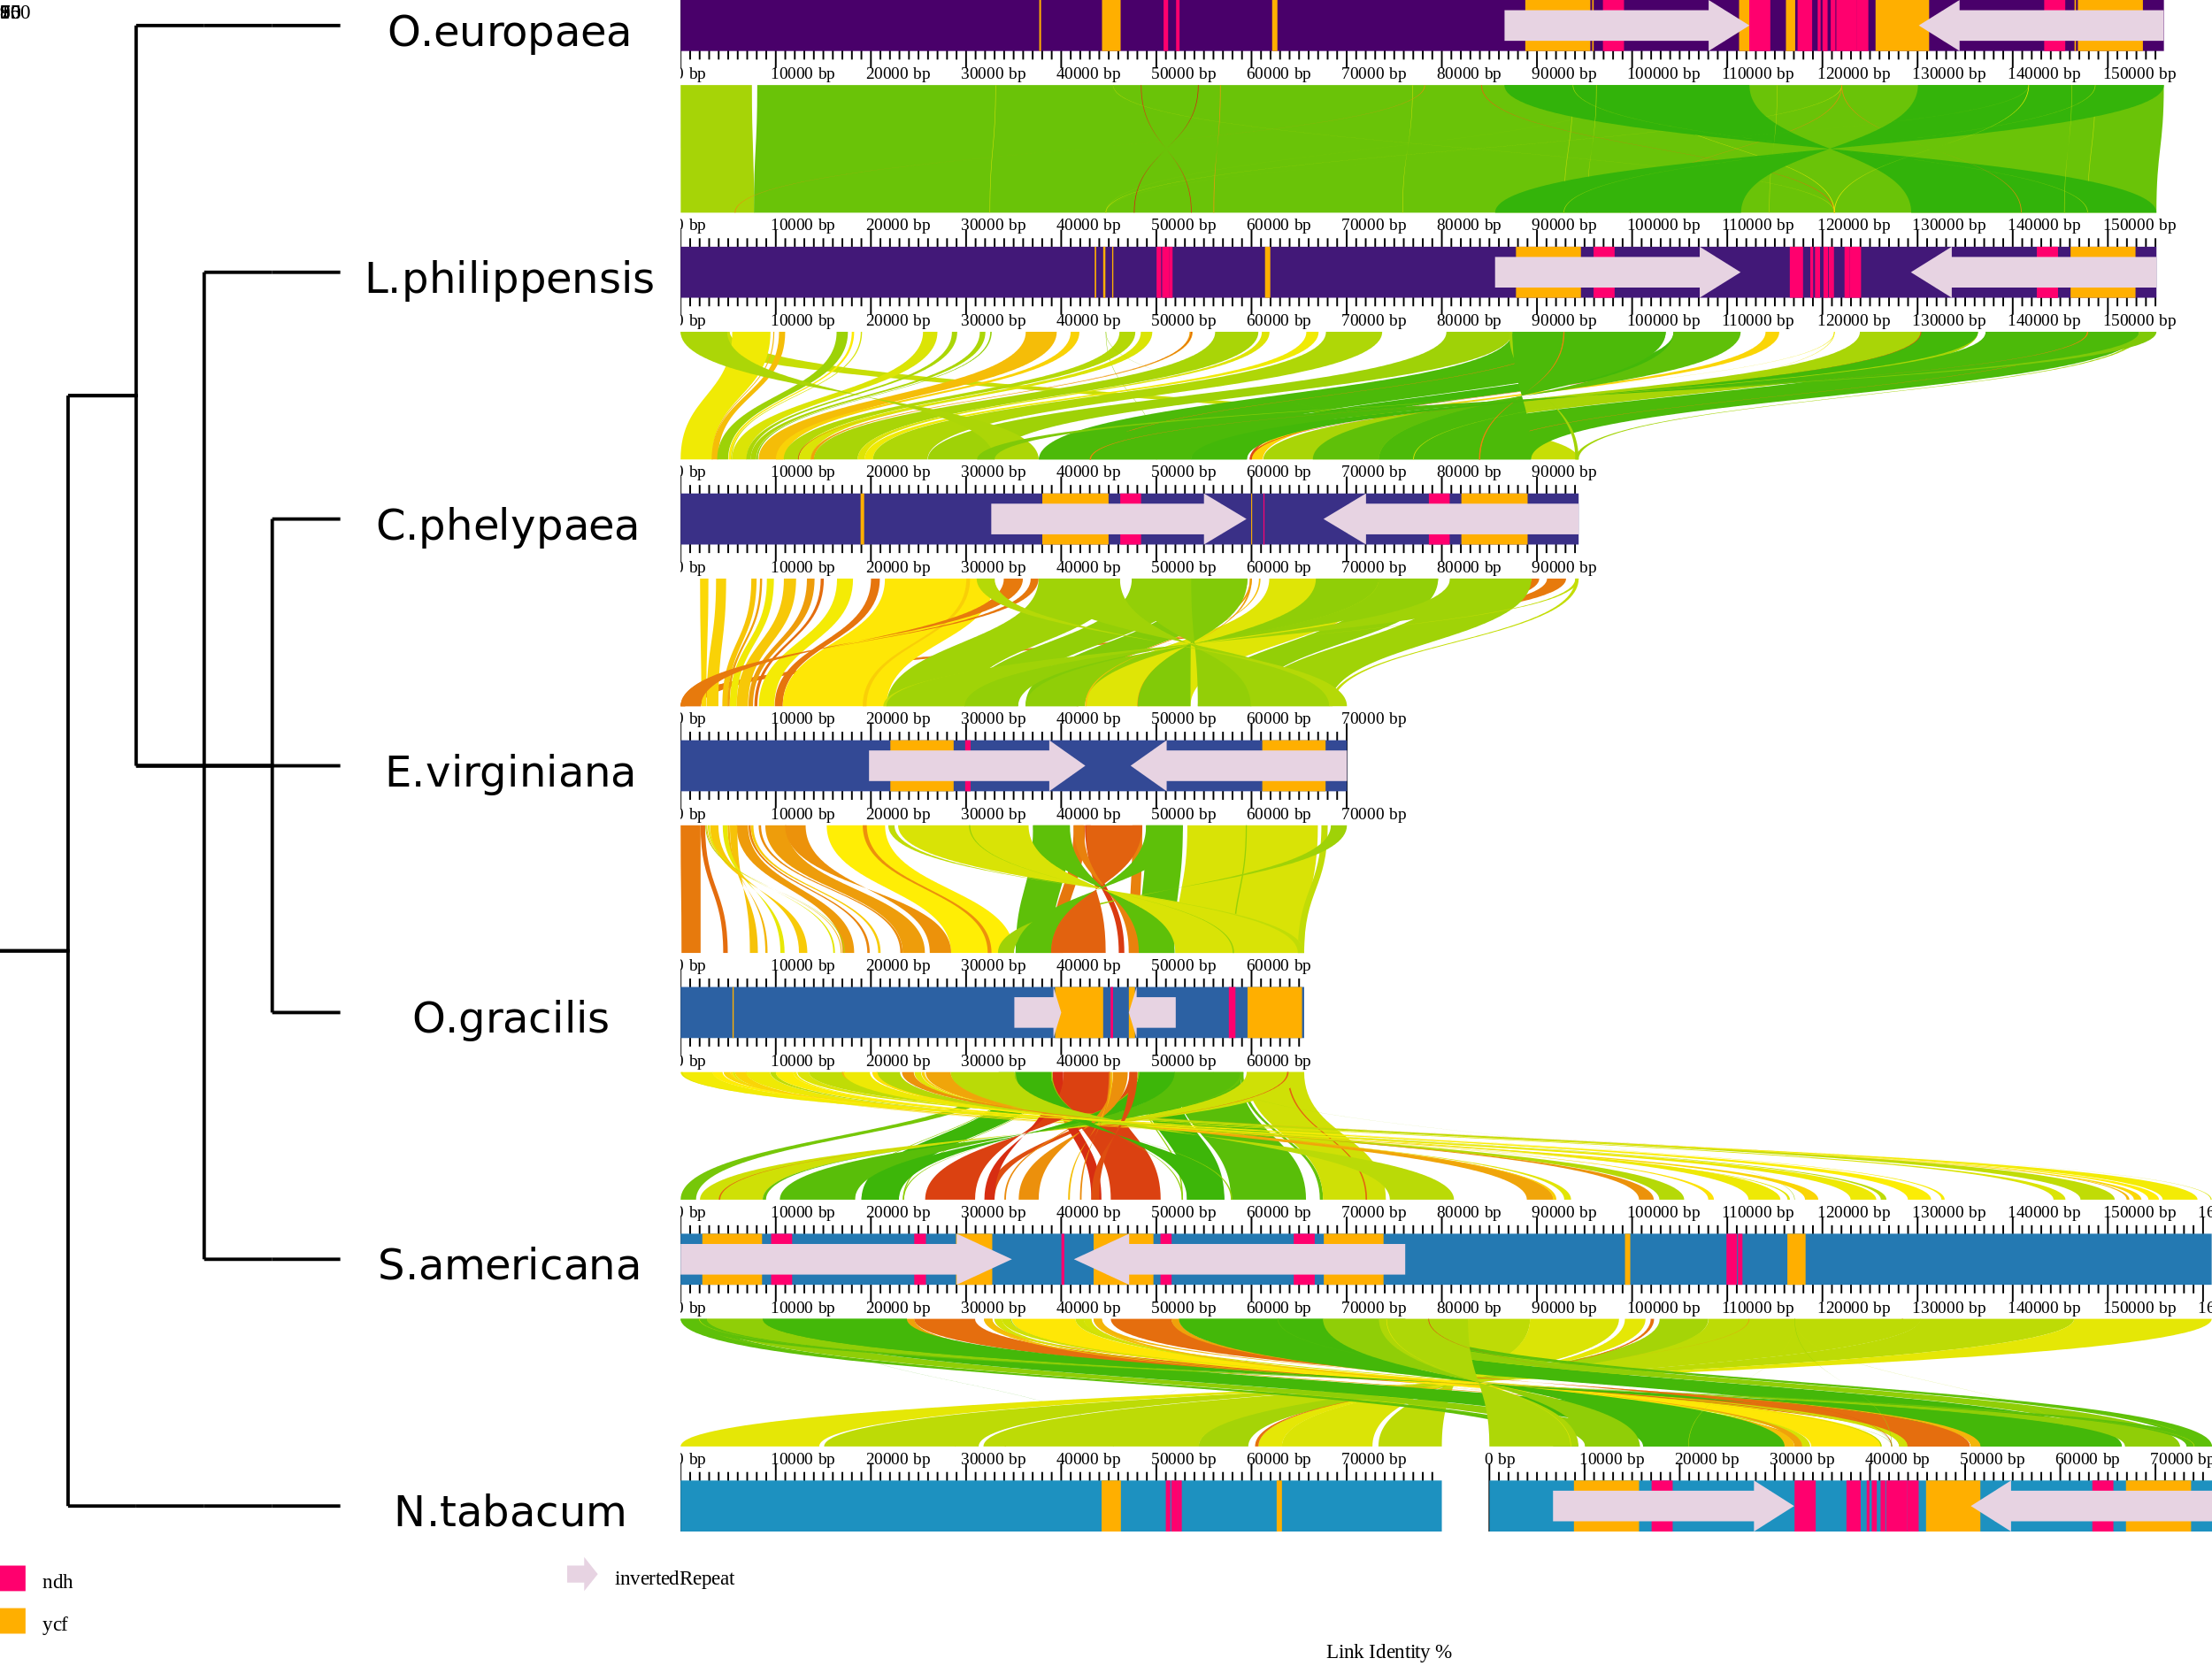
\includegraphics[width=10cm]{showLabels.png}
		\caption{The AliTV image using the default configuration.}
	\end{figure}
	
	\item As you can see seven chloroplast genomes and the alignments between adjacent genomes are visualized. The genome of \textit{N. tabacum} is splitted in two parts. 
	\item The phylogenetic tree represents the relationship between the analyzed genomes.
	\item At the bottom a legend shows the biological features and the scale of the link identity.
\end{itemize}

\paragraph*{Create figure}
\begin{itemize}
	\item For using the figure you have to download it. Click \texttt{Import \& Export -> Save SVG} for saving the picture.
	\item Open the folder where you saved the AliTV image and open it with your favourite image-viewer.
\end{itemize}

\paragraph*{Change the genome orientation}
\begin{itemize}
	\item The direction of \emph{S. americana} is the opposite in contrast to the adjacent genomes, because the alignments between them are twisted. Therefore AliTV provides the option to set the sequence orientation forward or reverse in order to obtain a clearer comparasion. 
	\item A context menu appears by right-clicking the genome of \emph{S. americana}. Select \texttt{Change orientation}.
	\item With an easy mouseclick you have changed the orientation of \emph{S. americana} and can now analyse the alignments between this and the adjacent genomes.
	
	\begin{figure}[H]
		\centering
		
\includegraphics[width=10cm]{reverse.png}
	\end{figure}
	
\end{itemize}
	
\paragraph*{Set tree configurations}
\begin{itemize}
	\item In the current settings the phylogenetic tree of the analyzed plants is presented. AliTV provides easy options for changing the tree layout.
	\item Choose the tab \texttt{Phylogenetic tree} on the HTML page.
	\item Here you can decide wether the tree is drawn or not. For the next few steps it is easier if the tree is not shown. Therefore make the checkobox unchecked.
	\item Submit the changes with \texttt{Apply}
	\item Now the phylogenetic tree is hidden. You can easy show him by checking the checkbox again.
\end{itemize}

\paragraph*{Change the genome and chromosome order}	
\begin{itemize}
\item If you want to compare \emph{N. tabacum} to \emph{L. philippensis} AliTV provides an easy option for changing the genome order.
\item You can change the order by right-clicking \emph{N. tabacum}. The context menu appears. Select \texttt{Move down}. Now \emph{N. tabacum} swapped its position with the genome below. So you can easy compare \emph{N. tabacum} with \emph{L. philippensis}

	\begin{figure}
		\centering
		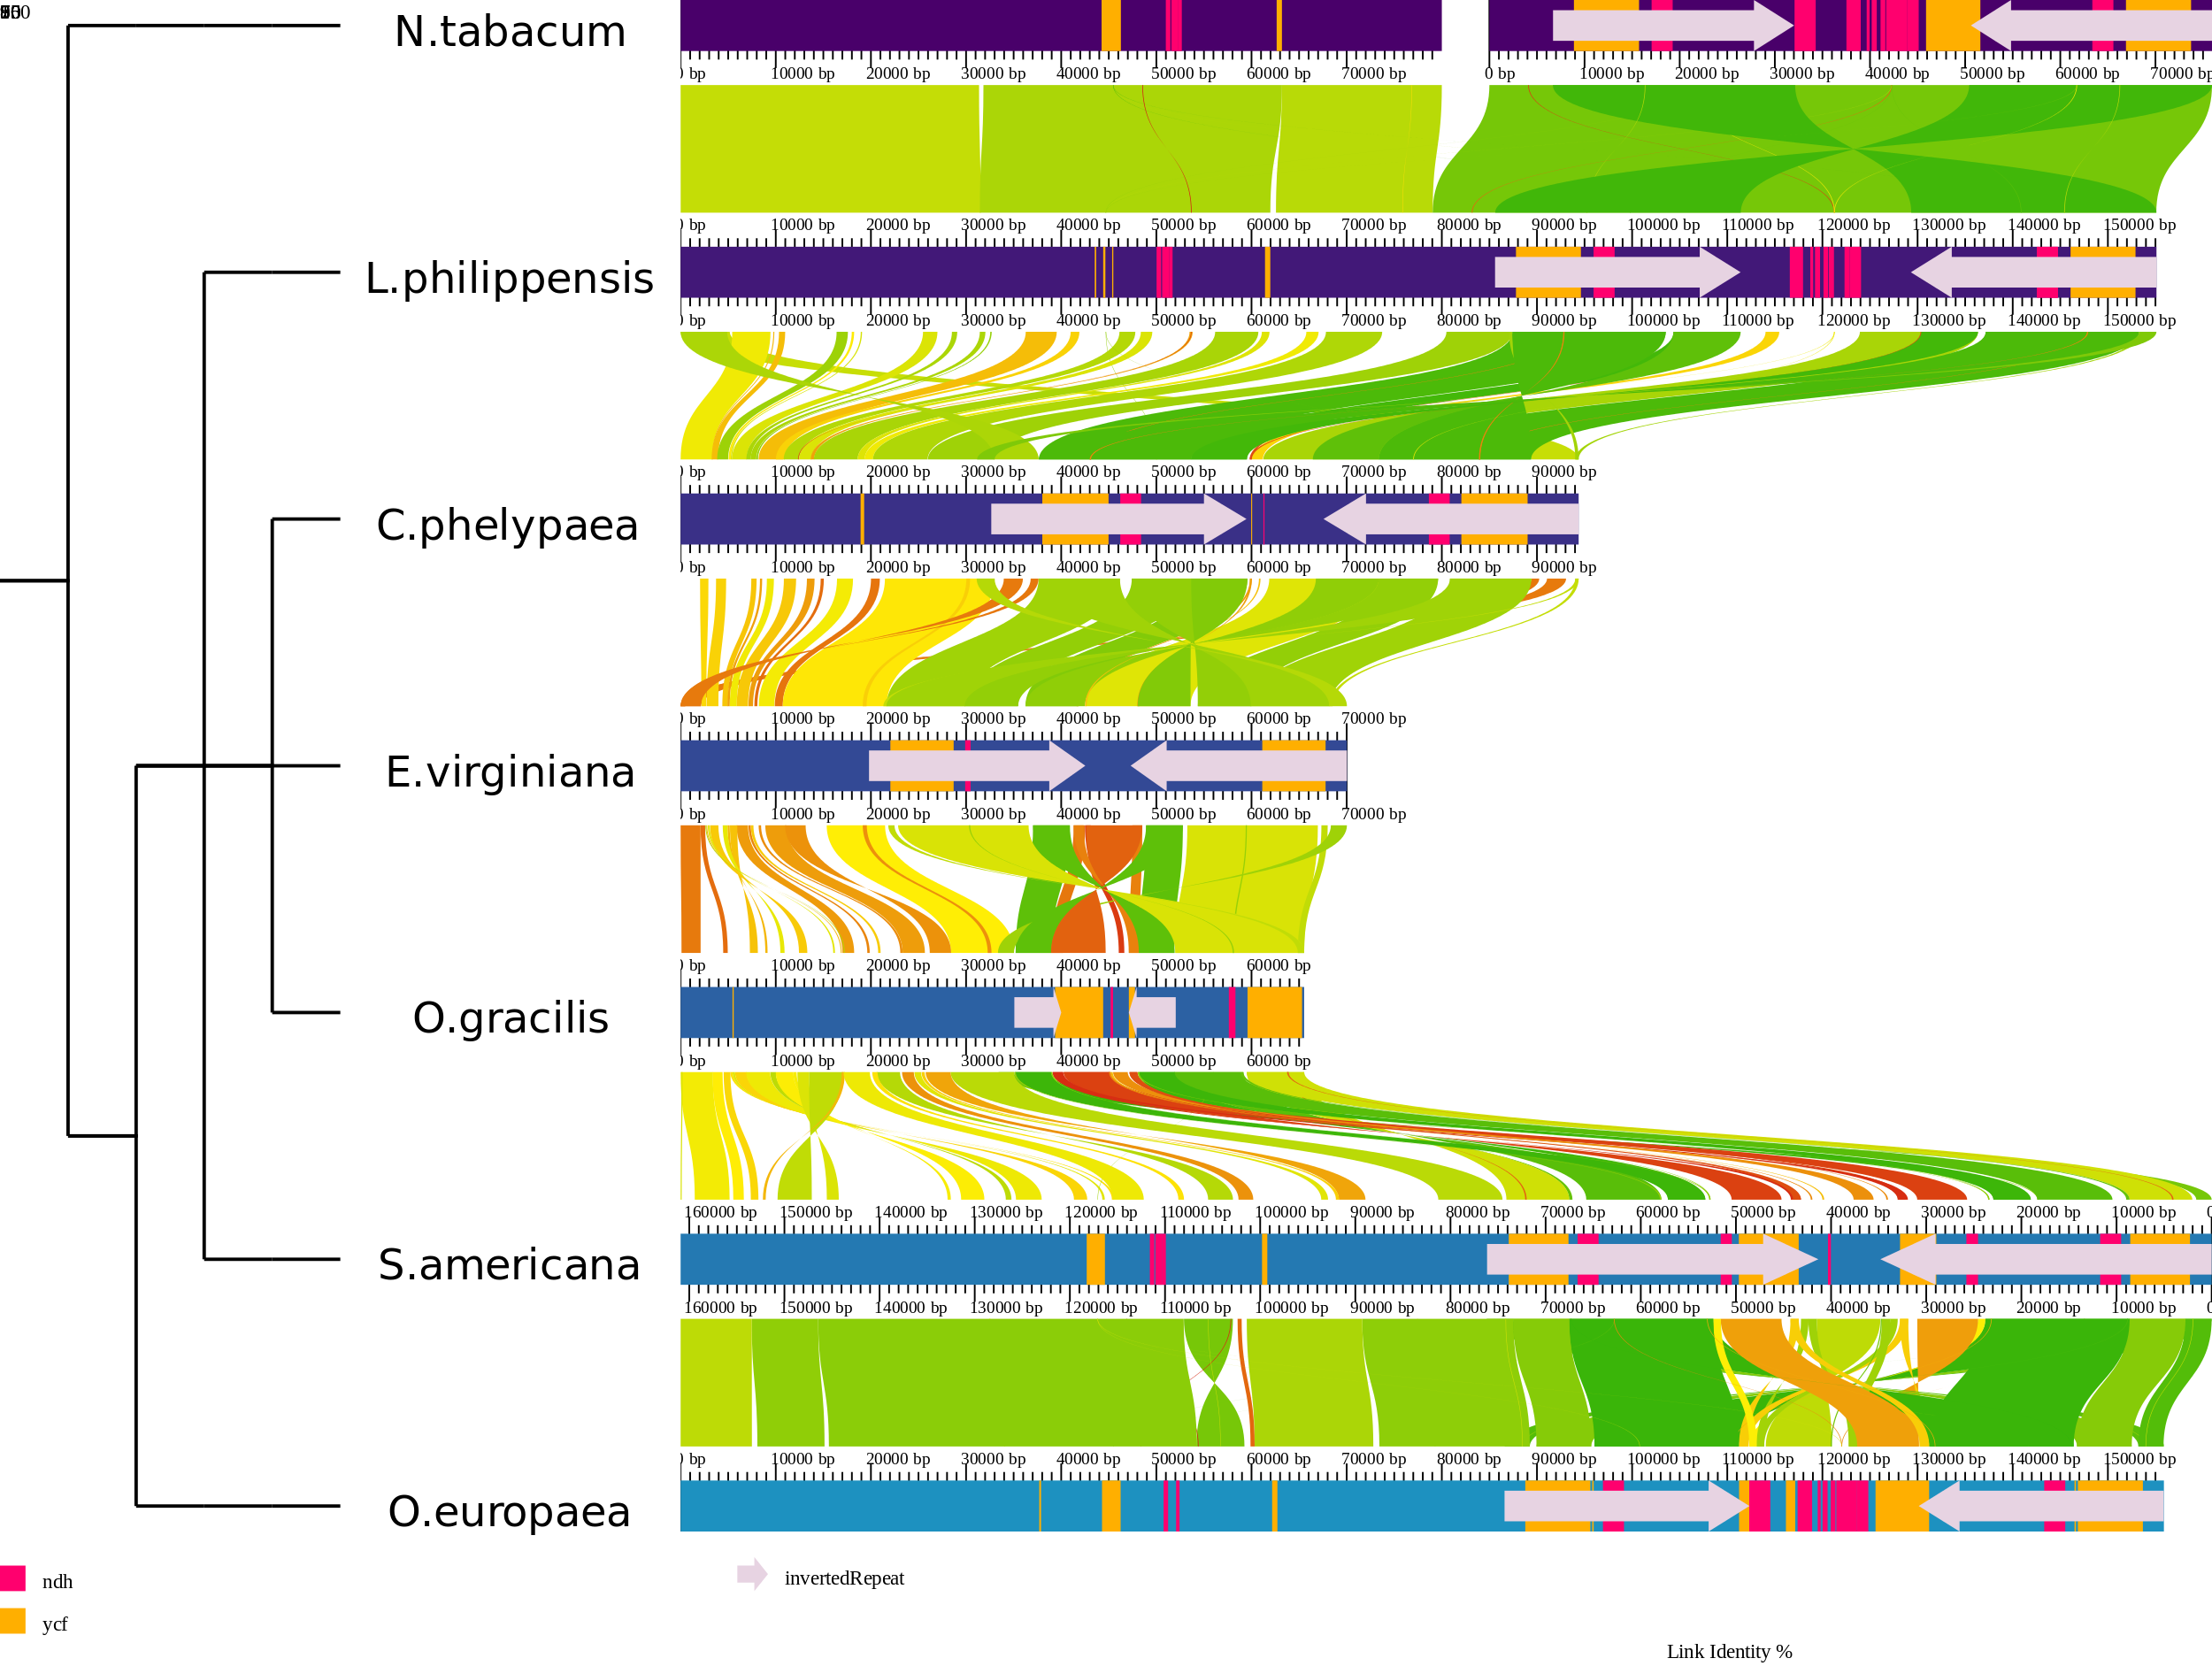
\includegraphics[width=10cm]{swap1.png}
		\caption{}
	\end{figure}
	
	\item As you can see the order of the phylogenetic tree has changed too. Its important to know that if the tree is drawn you can only swap genomes within the tree order. If the genome order is not concordant with the tree order the tree is hidden and a warning appears.
	
	\begin{figure}
		\centering
		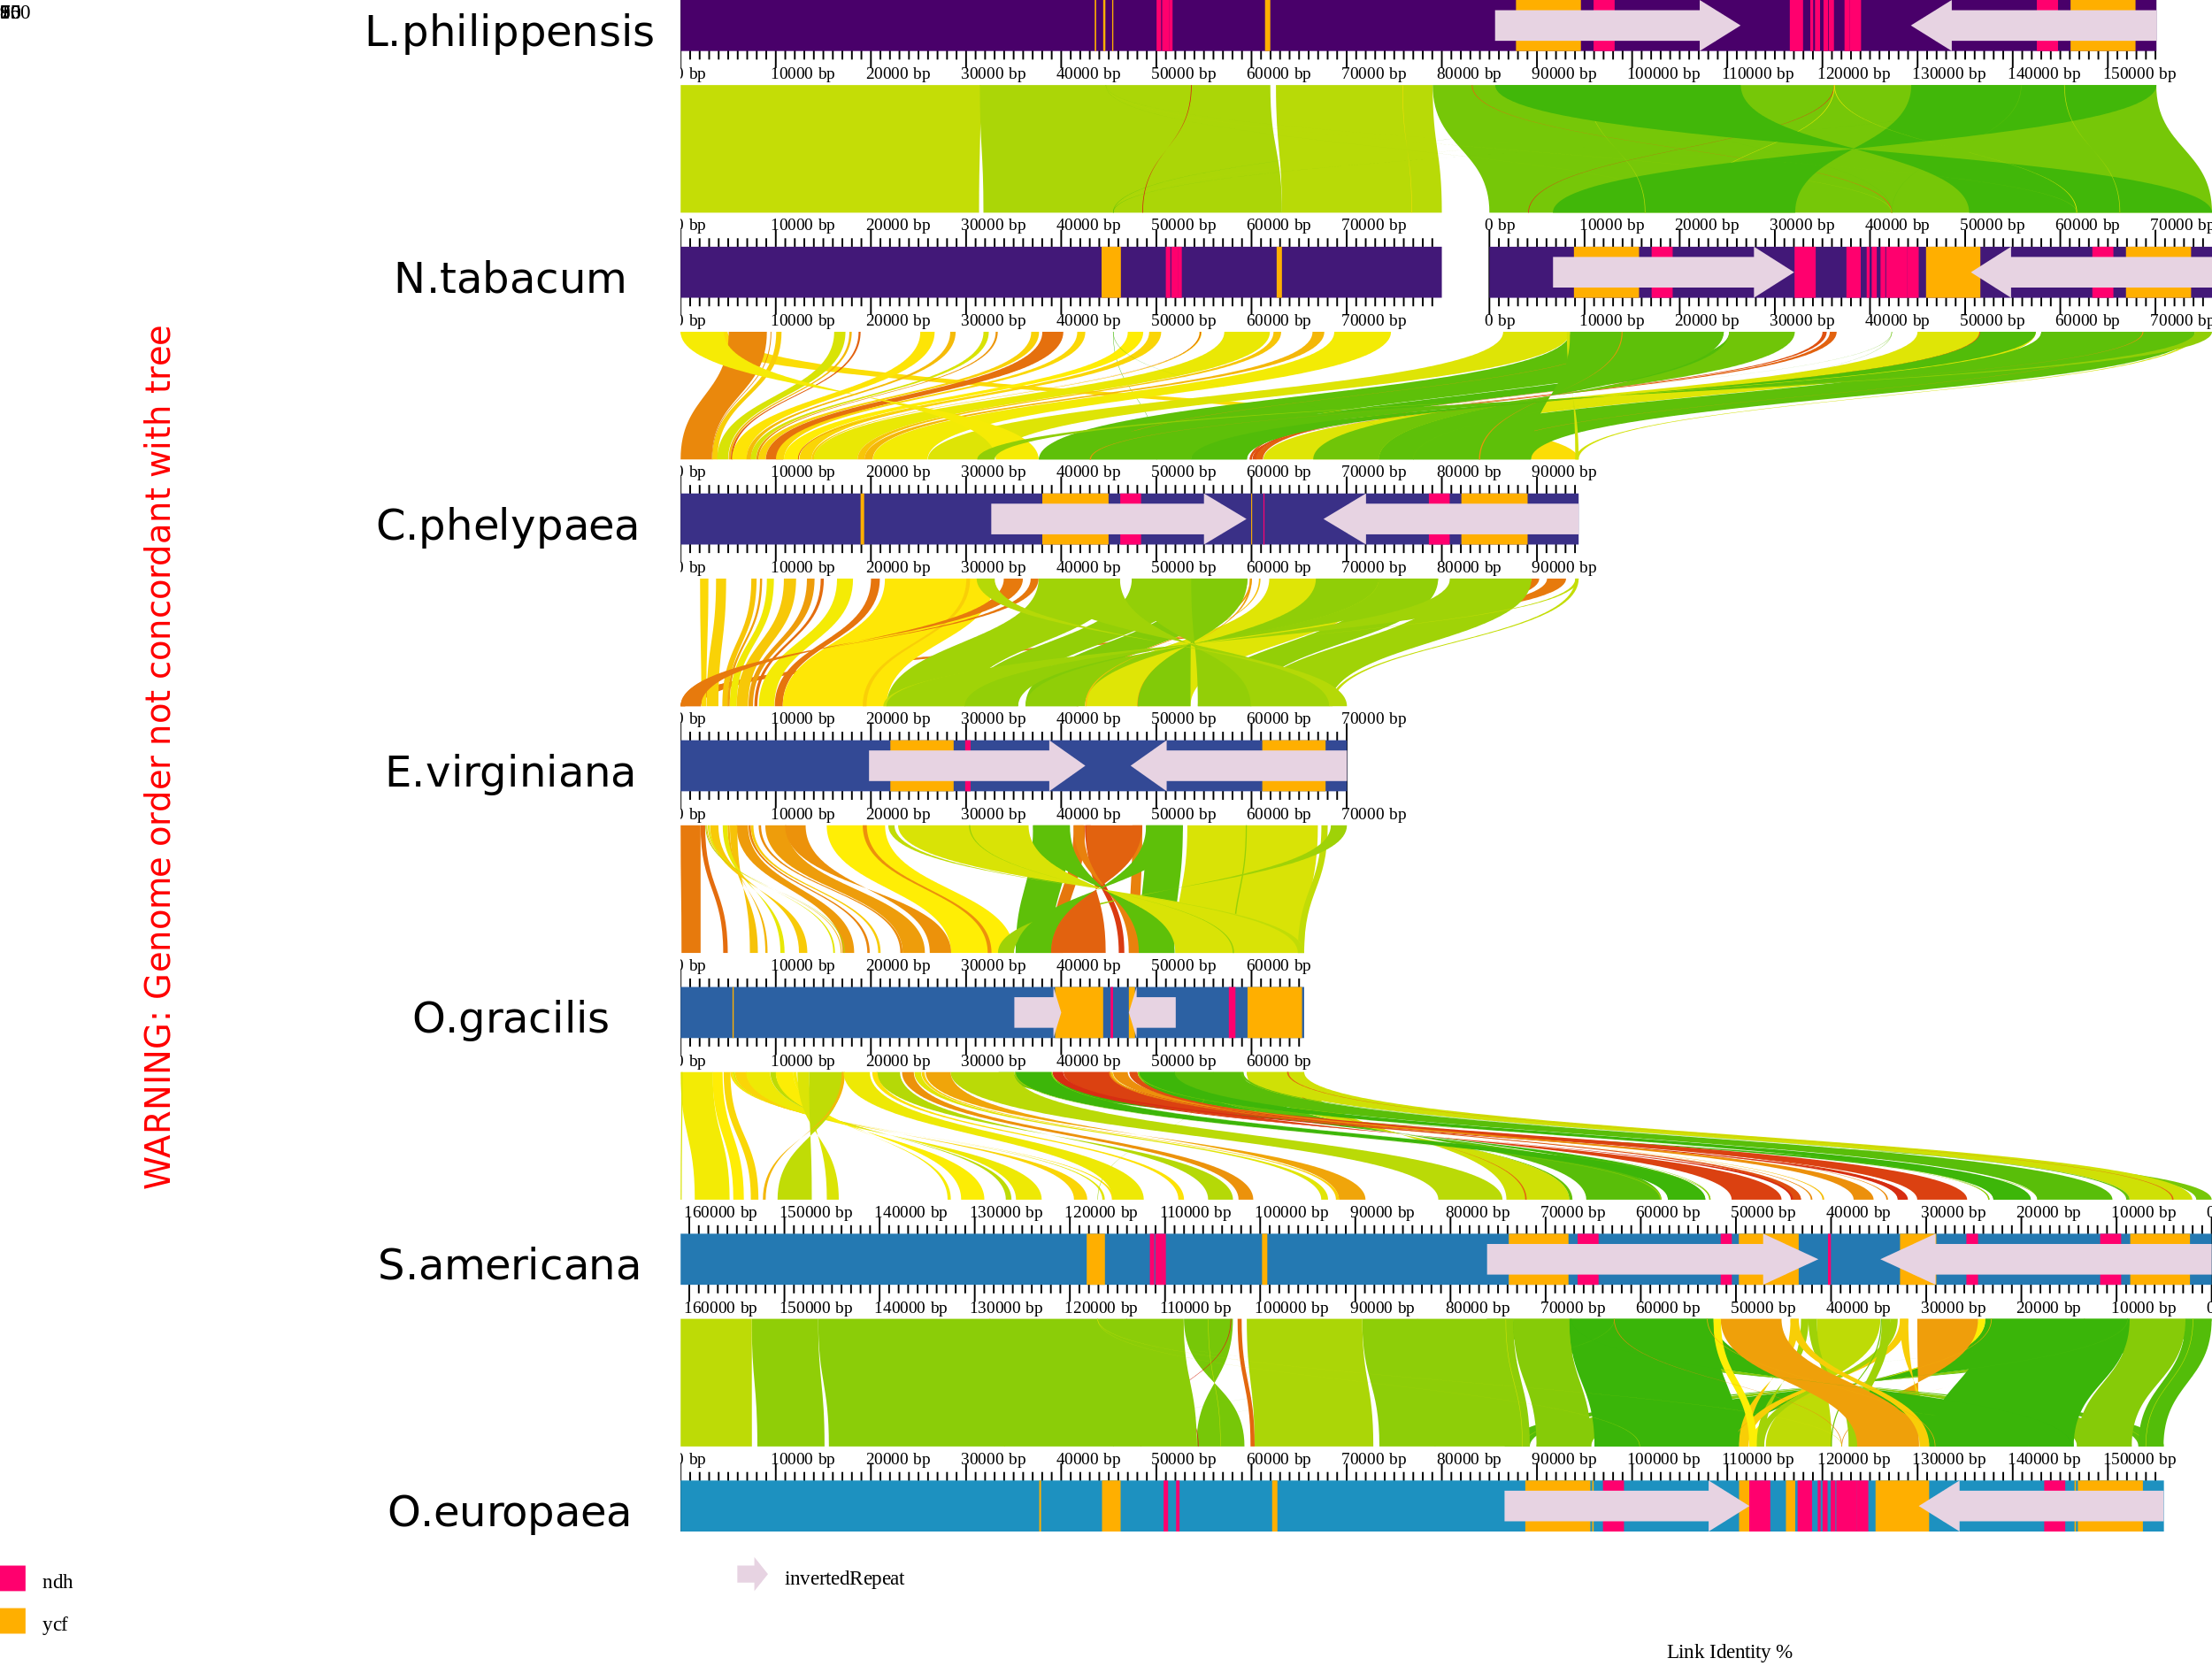
\includegraphics[width=10cm]{warn.png}
		\caption{}
	\end{figure}
	 
	\item For changing the order of chromosomes within a genome (for example \emph{N. tabacum}) you select the chromosome which you want to resort. In the contextmenu select \texttt{Move right} or \texttt{Move left}.
	\item When you want to save the image with the current settings you can download it as described in Create Figure.
\end{itemize}

\paragraph*{Filter links by identity and length}
\begin{itemize}
	\item For a biological analysis it may be helpful to filter links by their identity or length. AliTV offers both options for analyzing the image easy and interactive.
	\item Choose the tab \texttt{Filtering} on the HTML page.
	\item For filtering links you use the sliders. Set the range of the identity slider on 85\% to 100\%. Submit your changes with \texttt{Apply}.
	\item As you can see some of the red and orange colored links are not shown because their identity is less than 85\% and so they are filtered.
	
	\begin{figure}[H]
		\centering
		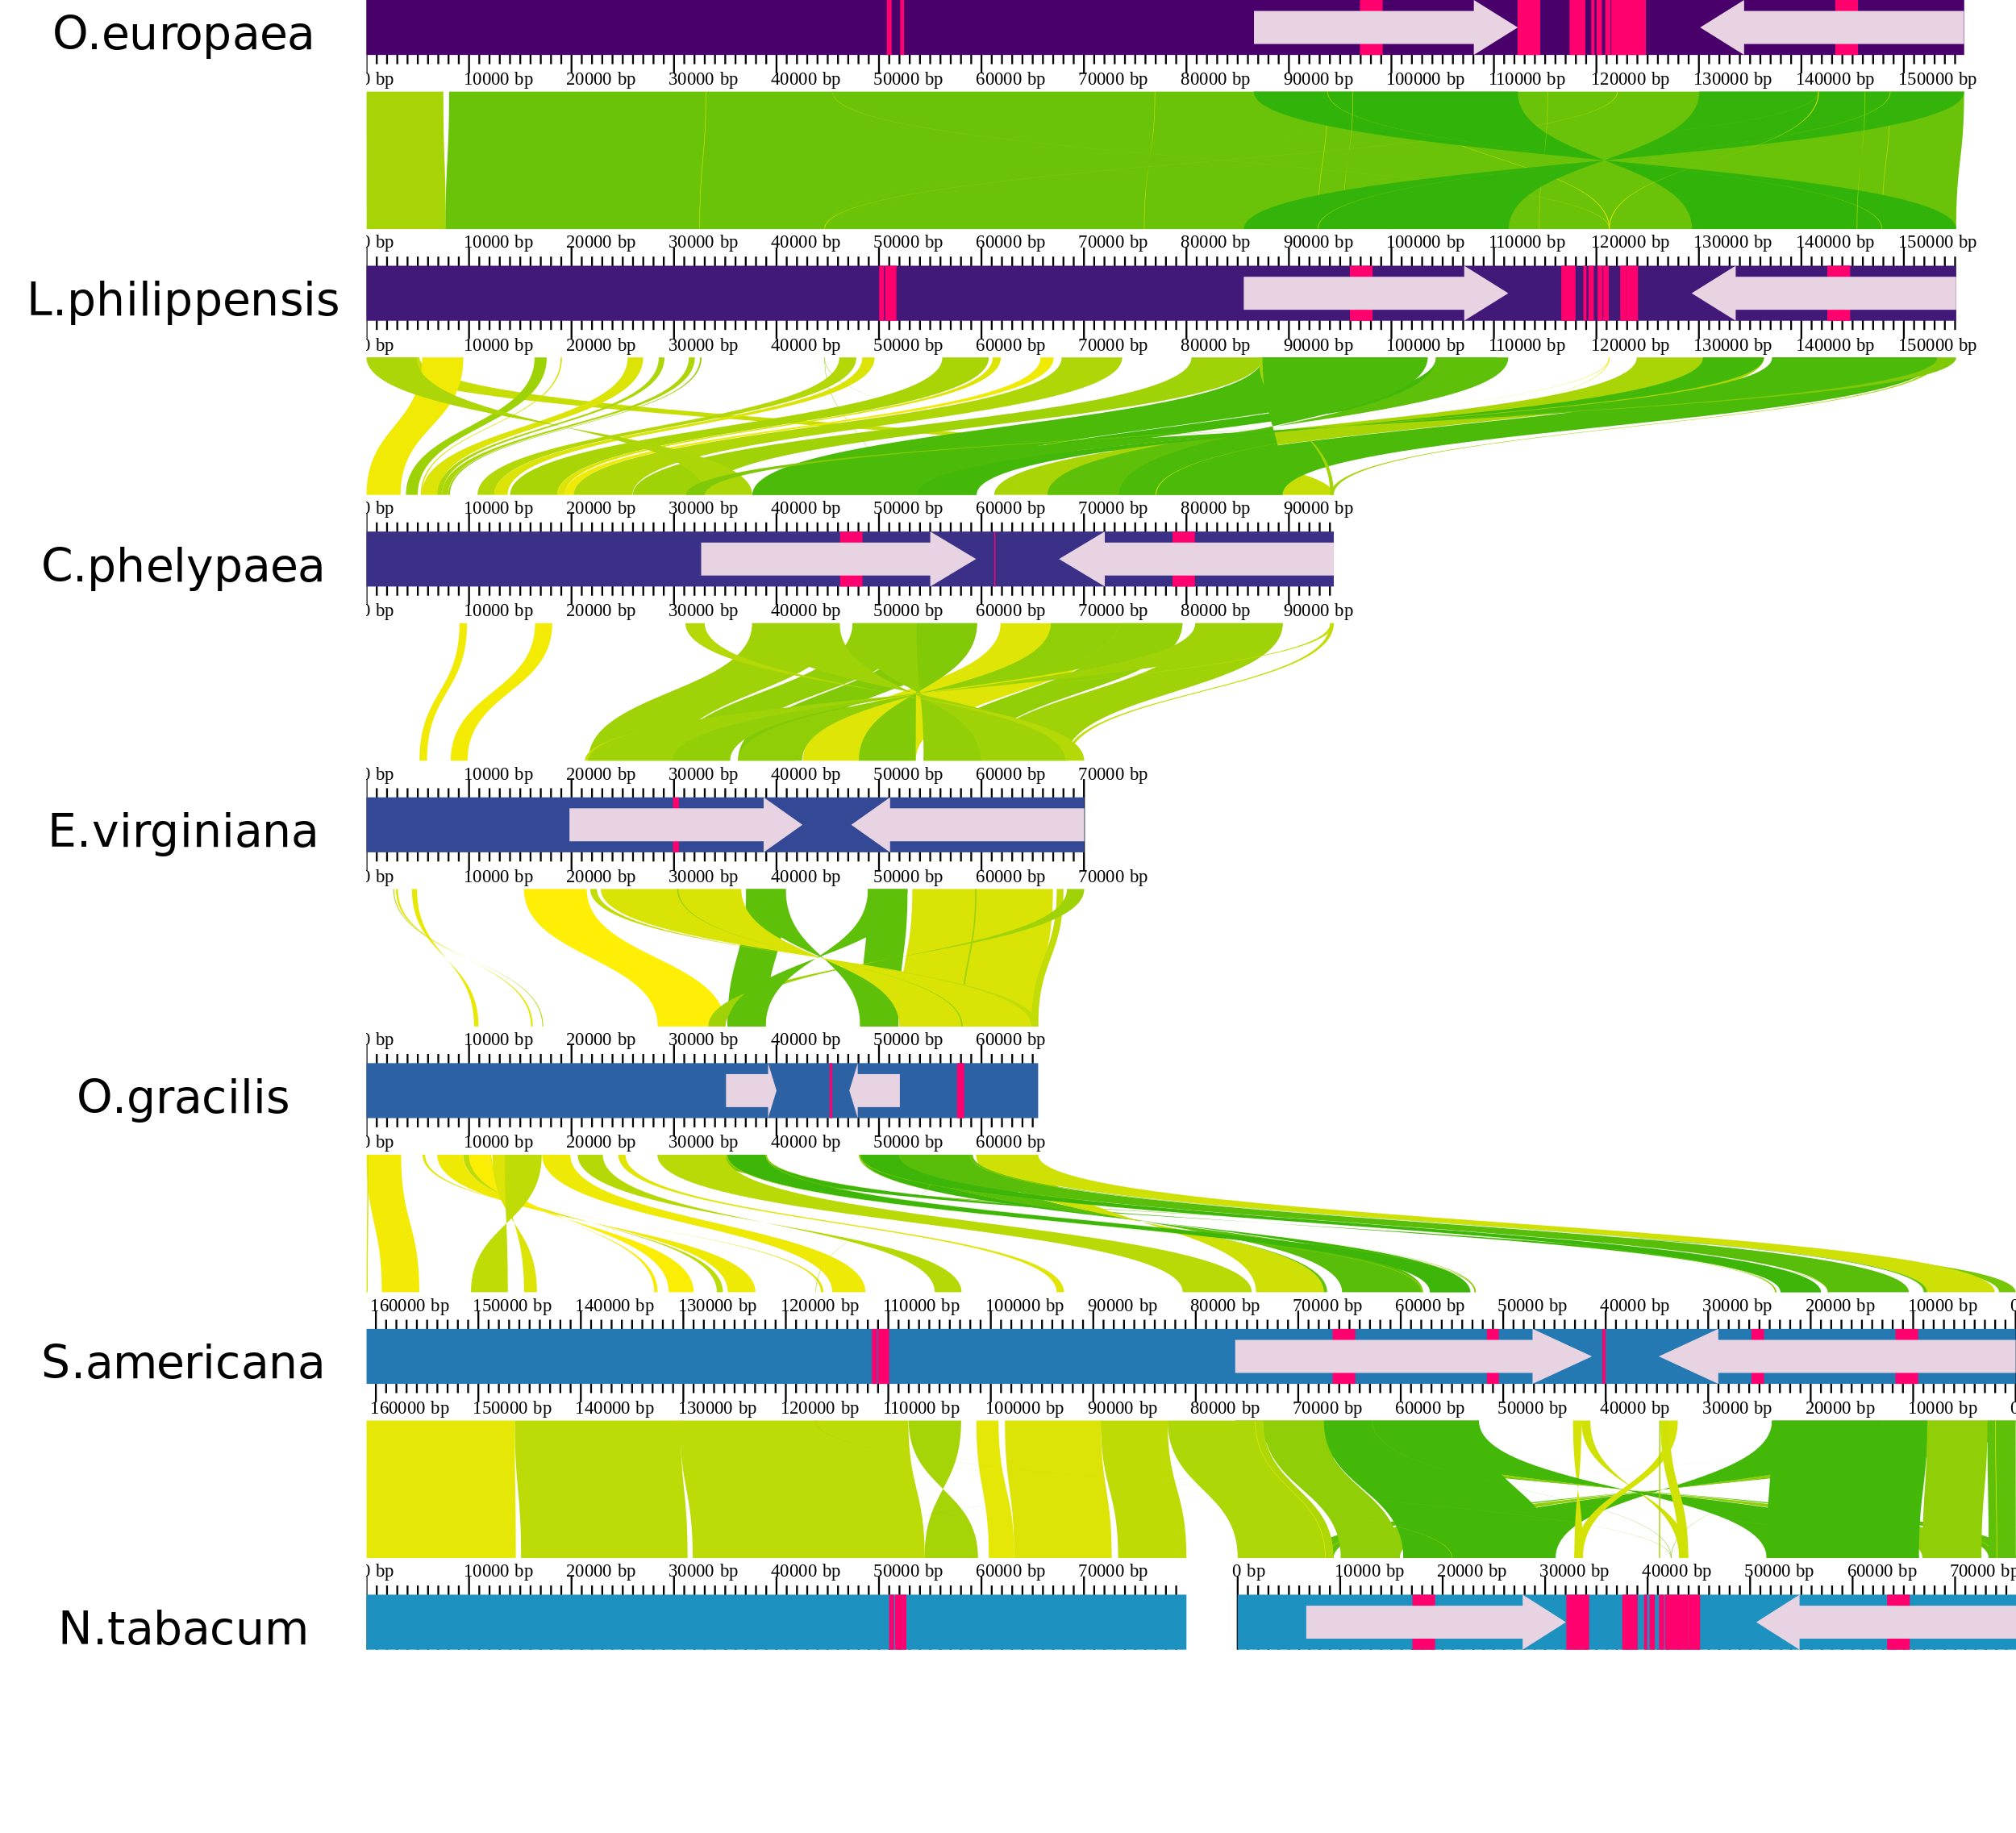
\includegraphics[width=10cm]{filterLinks.png}
		\caption{}
	\end{figure}
	
	\item In the same way links can be filtered by their length. So try it and have fun with this nice sliders!
\end{itemize}

\paragraph*{Change graphical parameters}
AliTV provides many ways to customise the image. The following list only shows a few examples. For more information checkout \textbf{Features of AliTV} or try it by yourself.

\subparagraph*{Setting the layout}
\begin{itemize}
	\item Select \texttt{Layout Settings} and choose your favourite layout (circular or linear).
	
	\begin{figure}[H]
		\centering
		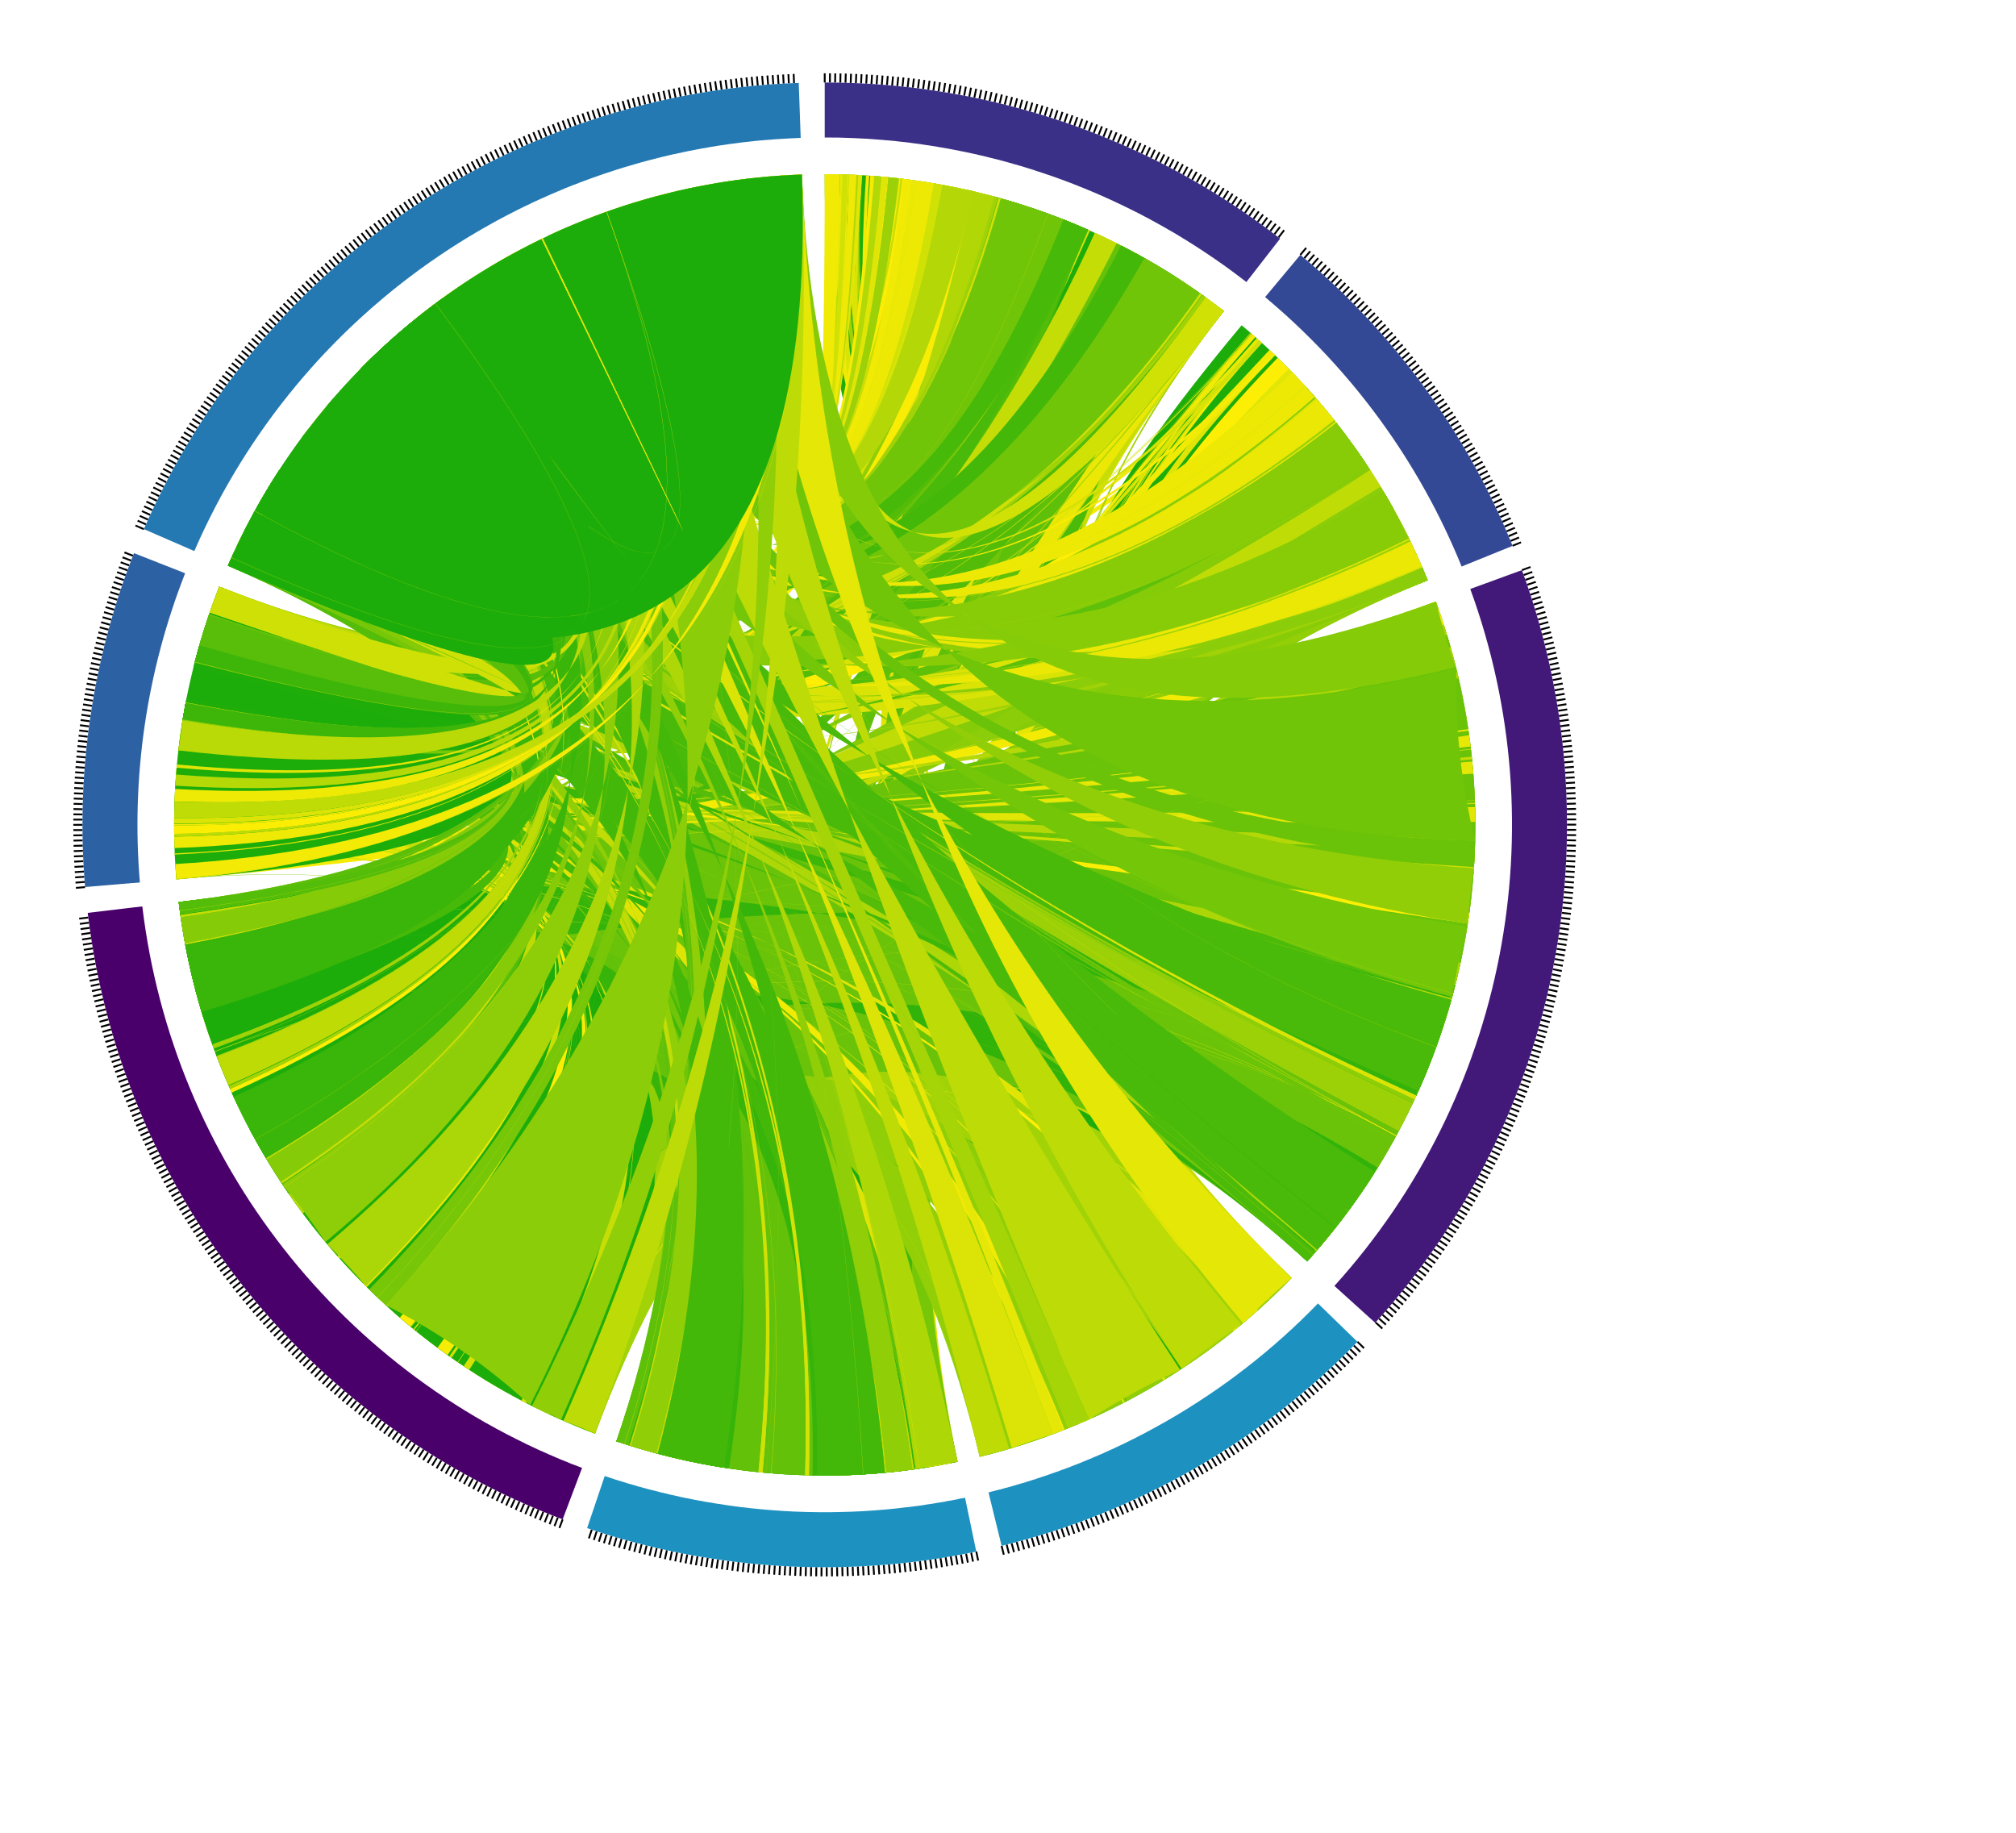
\includegraphics[width=10cm]{circular.png}
		\caption{}
	\end{figure}

	 \item At the moment the circular layout is not the development stage of the linear layout. Therefore the most options and interactive functions are not working if you use it.
\end{itemize}

\subparagraph{Coloring the chromosomes}
\begin{itemize}
	\item With AliTV it is possible to change the color range of the presented genomes, the color of features and labels.
	\item Select \texttt{Layout Settings} and define a new start and end color by using the color picker. It is also possible to type in the Hex or RGB value of your favourite color.
	\item If you use \#00ffc2 for color 1 and \#ff8a00 for color 2 you get the following crazy AliTV image.
	\begin{figure}[H]
		\centering
		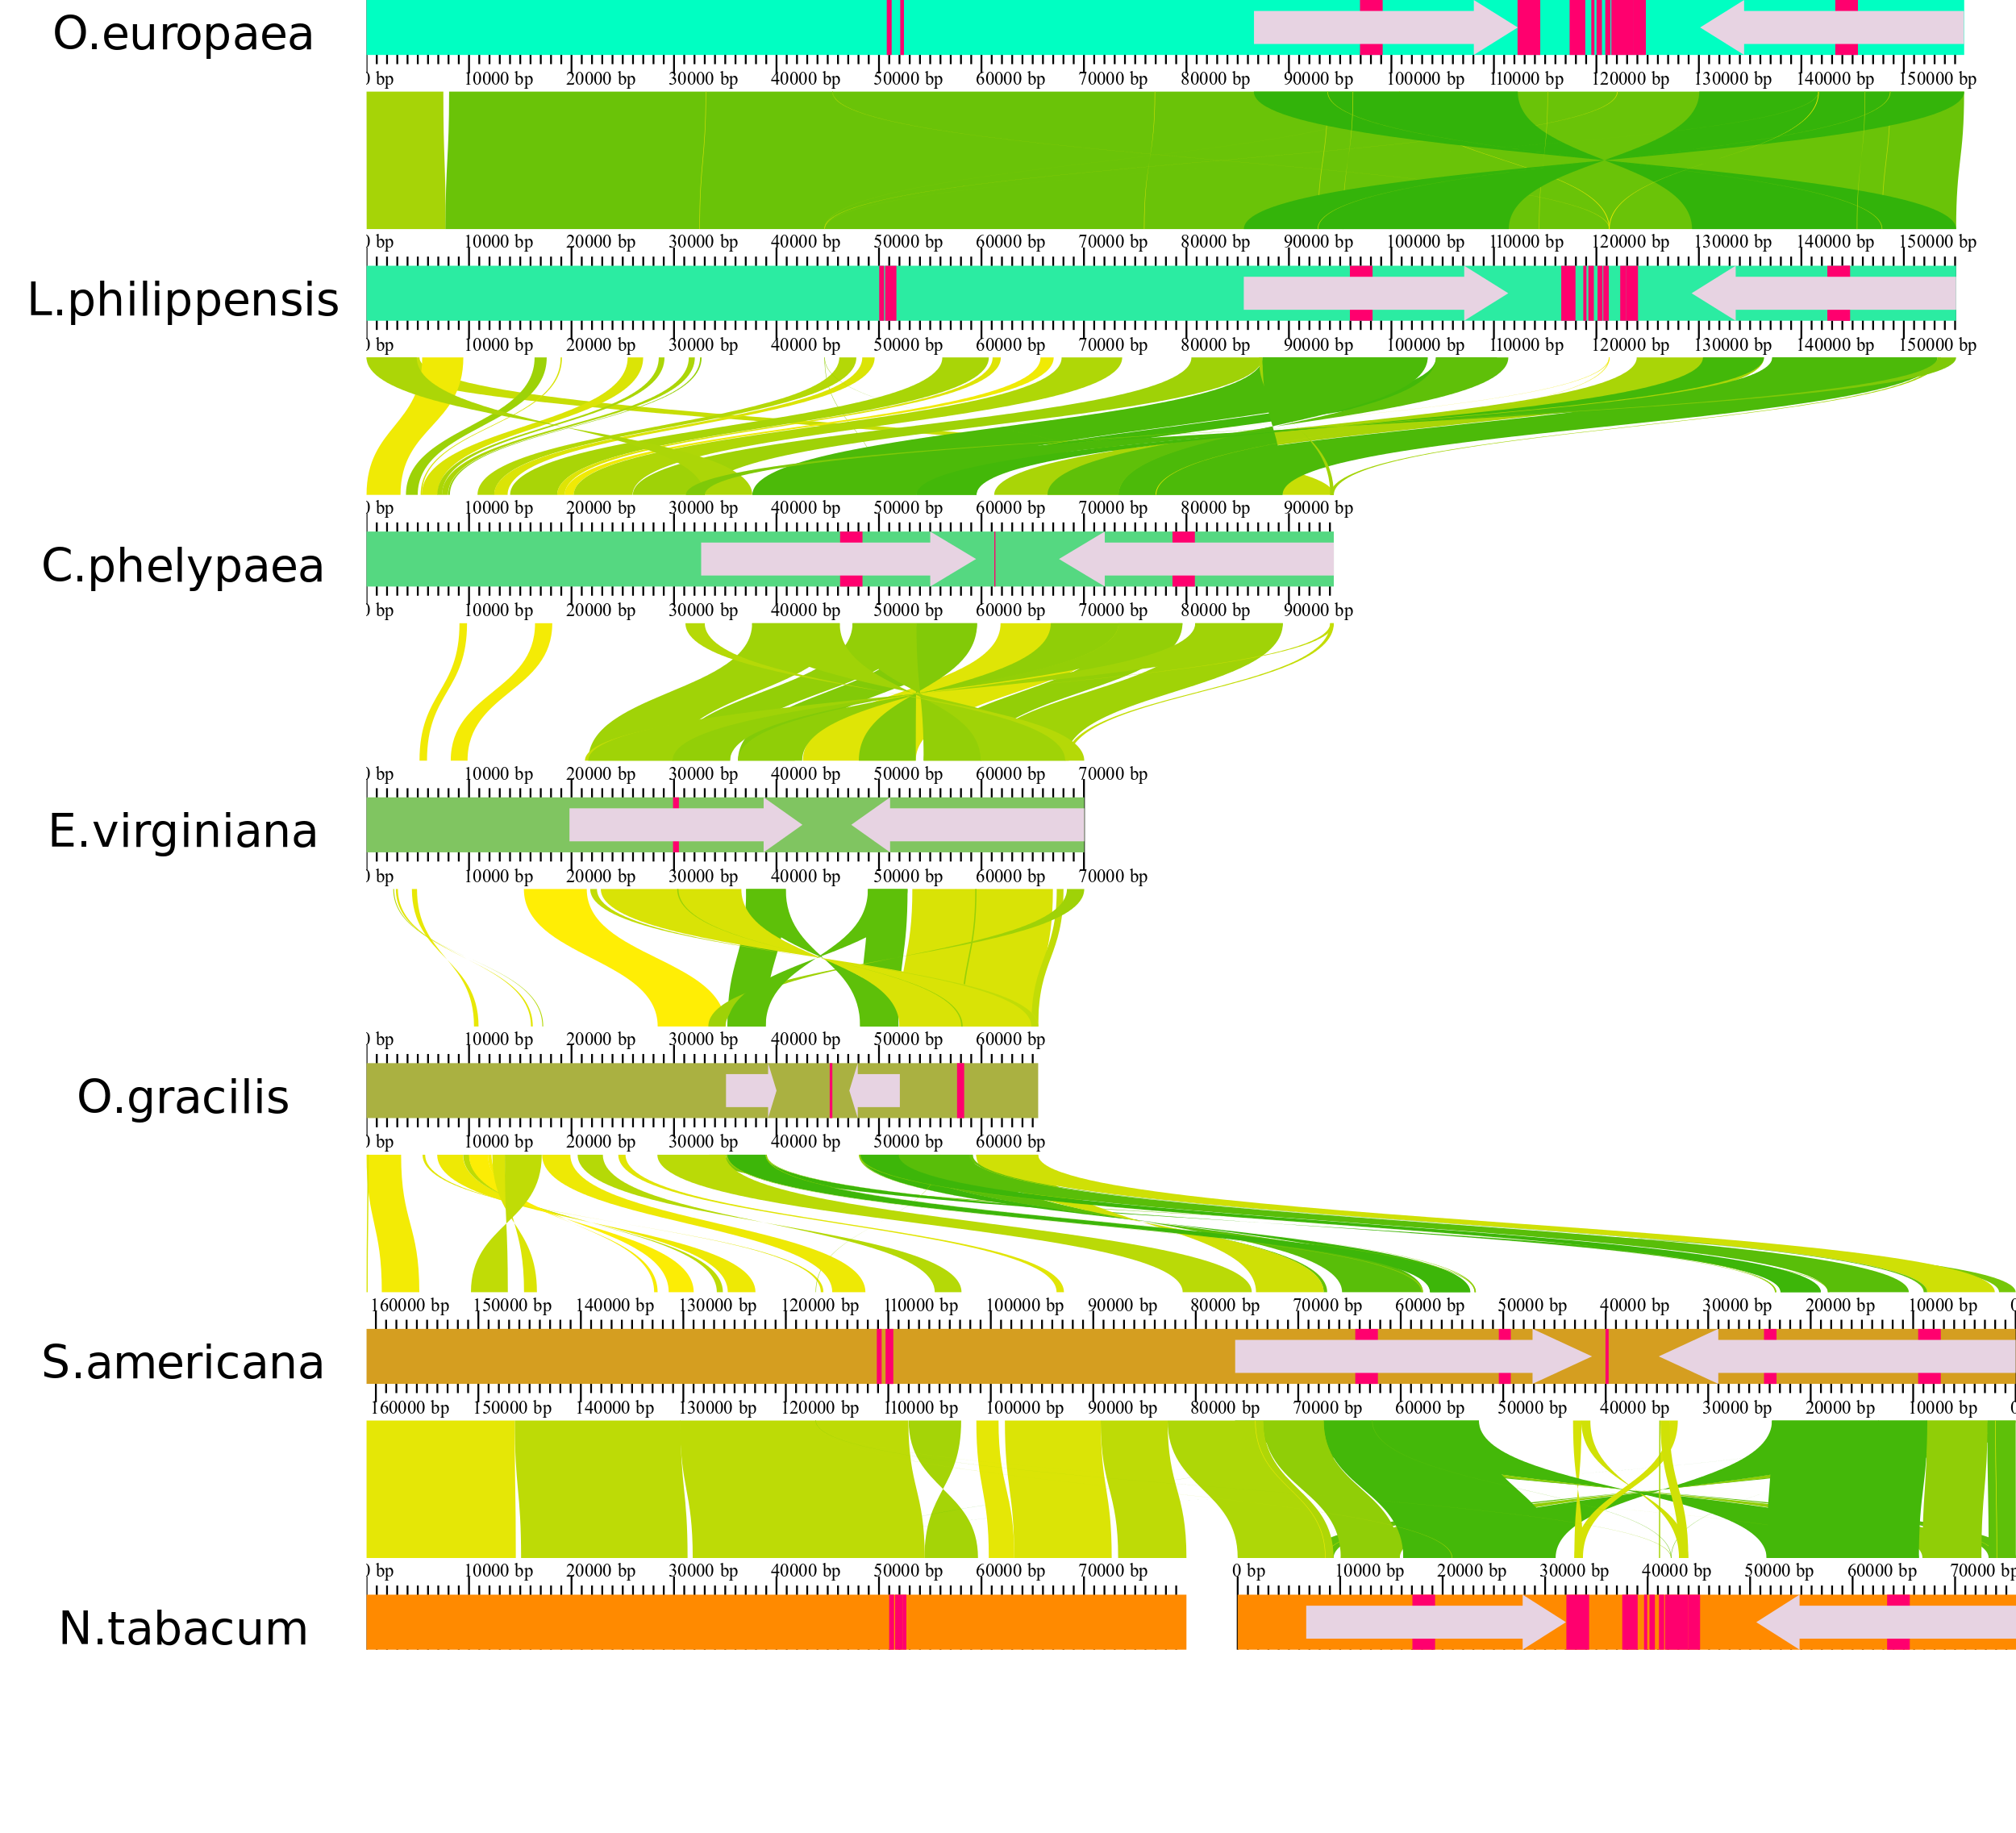
\includegraphics[width=10cm]{crazy.png}
		\caption{Setting new values for the genome color.}
	\end{figure}
\end{itemize}

\subparagraph*{Scaling the chromosomes}
\begin{itemize}
	\item If you want to change the default scaling of the sequences select \texttt{Layout Settings} and type in a new tick distance in bp. 
	\item The labeling of the ticks is changing as well, because every tenth tick is labeled by default. When you want to change the tick labels you can type in their frequency in the current tab.
	\item If you set the tick distance to 10000bp and the label frequency to 3 you get the following image.
	\begin{figure}[H]
		\centering
		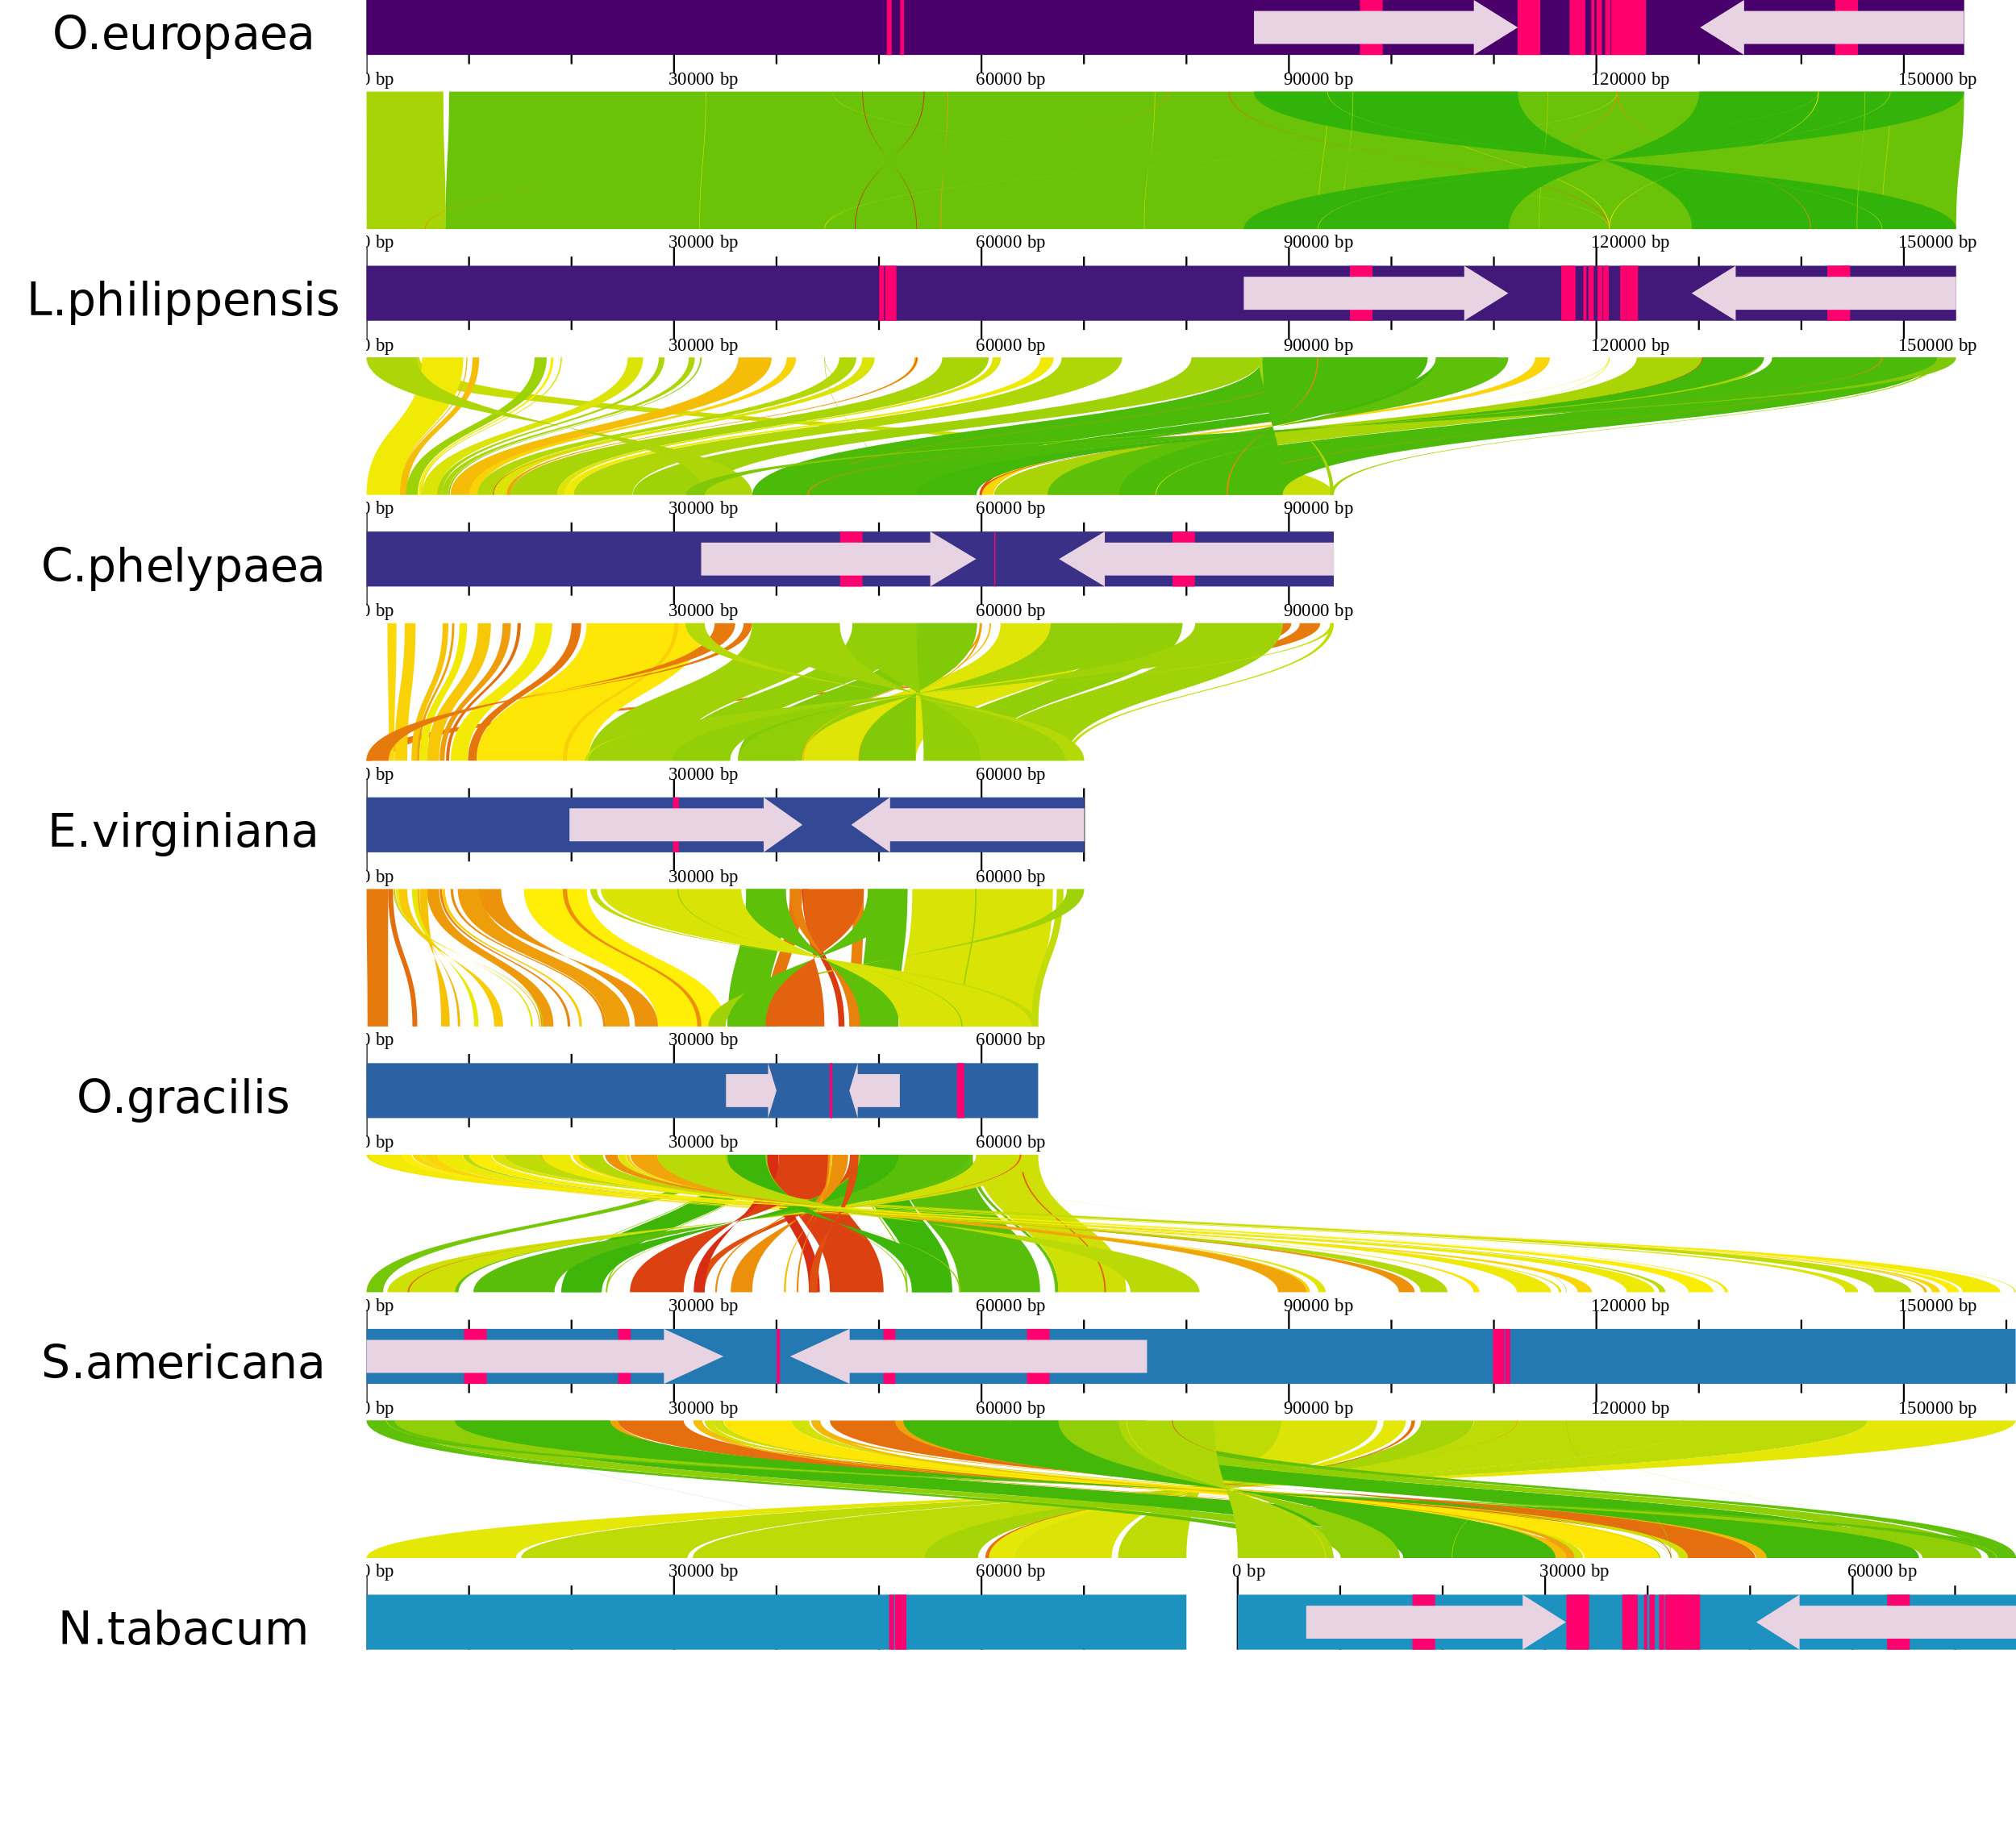
\includegraphics[width=10cm]{newLabels.png}
		\caption{AliTV offers easy scaling of chromosomes.}
	\end{figure}
\end{itemize}

\subparagraph*{Zooming}
\begin{itemize}
	\item AliTV provides a function for zooming genomic regions. For using the zoom feature you can directly interact with the AliTV image.
	\item Drag the mousepointer on the genome region you want to zoom. In this example we want to analyze the inverted repeat IrA of \textit{L. philippensis}.
	\item A rect selection appears. Drop it and you zoomed into the selected region.
	
	\begin{figure}[H]
		\centering
		
\includegraphics[width=10cm]{zoom.png}
		\caption{}
	\end{figure}
	
	\item You can reset the zoom by right-clicking onto the chromosome and select \texttt{Reset genome zoom/pan}.
\end{itemize}

\subparagraph*{Shifting}
\begin{itemize}
	\item For analyzing circular sequences it may be helpful to rotate them. Therefore go to \texttt{Advanced Settings}.
	\item Via the selection box you select the chromosome you want to shift. As you can see a button group appears next to the selected chromosome.
	\item By using the right or left arrow you shift the chromosome for a tick distance. If a link or a feature has an overlap it will be splitted into two parts.
	
	\begin{figure}[H]
		\centering
		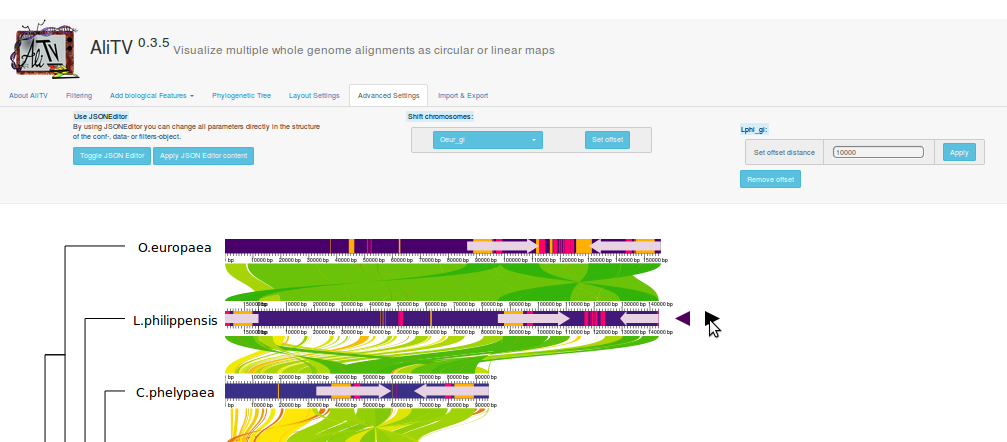
\includegraphics[width=10cm]{shift.png}
		\caption{Via the interface chromosomes can be shifted.}
	\end{figure}	
	
	\item For changing the offset distance type in a new value in the cooresponding input field.
	\item You can remove the offset by clicking \texttt{Remove Offset}. Now the button group is removed and the shifted chromosome is resetted.
	
\end{itemize}

\newpage
\section*{Features of AliTV}
\subsection*{Main Screen}
Above is the user interface of AliTV available on the HTML page when you generate the figure. The current version of AliTV is presented on the frontend.
\begin{figure}[H]
	\centering
	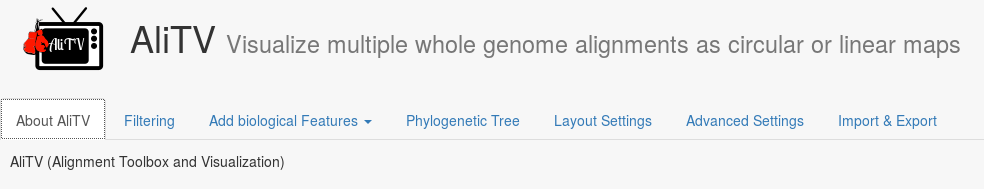
\includegraphics[width=14cm]{userInterface.png}
	\caption{User interface of AliTV}
\end{figure}
\paragraph*{About AliTV}
Contains information of the software as well as direct links to the demo version, the manual and the code documentation.

\paragraph*{Filtering}
Will filter the alignments according to their identity and length by using the sliders. With \texttt{Apply} the changes are submitted.

On top of that this tab contains the information about all links, features or chromosomes which are hidden in the current settings. By using the selectors you can show a specifc hidden element again. With clicking \texttt{Restore Feature/Chromosome/Link} the changes are submitted.

\paragraph*{Add biological features}
AliTV provides the possibility to show genes, inverted repeats, repeats and N-stretches by default. If you assigned the necessary data to AliTV you can configurate them by using this feature. 

With the checkboxes genes are shown, hidden or labeled. You can choose between a rect or an arrow and you can color them by using the colorpicker. With \texttt{Apply} you submit the changes.

It is the same procedure for inverted repeats, repeats and N-stretches. But it is important that you assign the data to AliTV. Otherwise no biolgoical features are visualized.

With AliTV it is possible to visualize custom features like specific gene groups, t-RNAs and other crazy stuff you want to show on the chromosomes. 

Therefore you can type in the name of your custom feature group, select a form and choose a color. That's it! As you can see it is very easy to visualize every biological stuff with AliTV.

\paragraph*{Phylogenetic Tree}
Here you can decide wether the phylogenetic tree is drawn or not. Moreover you can show the tree left or right to the alignments and you can change its width.

\paragraph*{Layout Settings}
All parameters that deal with color, size and layout of the AliTV image can be setted here. You can change the image size, the colors of chromosomes and links and the labels.

\paragraph*{Advanced Settings}
AliTV uses the \texttt{JSONEditor} in order to offer you the possibility for changing parameters, filters and data structure directly next to the figure. By clicking \texttt{Toggle JSONEditor} the editor appears at the bottom of the HTML page. 

First you see the structure of an AliTV object with \texttt{data, filters} and \texttt{conf}. \texttt{data} contains the data and it simply consists of \texttt{karyo, links, features (optional)} and  \texttt{tree (optional)}. All graphical parameters like color, size, layout, etc. and other configuration for drawing the AliTV image are written in \texttt{conf}. Specific configurations like hidden chromosomes, links or features and the minimal and maximal link identity and length are assigned to \texttt{filters}. All modifications you made are submitted by clicking \texttt{Apply JSONEditor content}.

For more information about the object structure and the means of the variables check out the documentation of AliTV. If you have problems with the JSONEditor the following link may be helpful for you: \url{https://github.com/josdejong/jsoneditor/}.

By using \texttt{Advanced Settings} you are able to rotate chromosomes. This feature is important if circular chromosomes are analyzed. Maybe you want to rotate them, so AliTV provides you the possibility to shift every chromosomes you want. Therefore use the selection box. Select any chromosome you want and click \texttt{Apply}. As you can see the button group appears next to the selected chromosome. By using the right arrow you shift the chromosome in positive direction. Using the other one you shift it in negative direction. Remember if you change the orientation of the selected chromosome the effect of the buttons are interchanged.

\paragraph*{Import \& Export}
If you want to use the AliTV image you have to download it. With \menu{Save SVG} you can download the AliTV image as SVG and open it with your favourite image-viewer. Moreover you can export the current settings in the JSON format by selecting \menu{Save JSON}. It may be helpful if you cant to save the settings and use it some other time. Then you can import JSON data by clicking \menu{Import JSON}.

\end{document}
